\chapter{AnnotateMe - An Entity Disambiguation Framework}
\label{chap:annotateme}
%Intro to the chapter
The work carried out by this research study can be logically divided into two parts that are closely interconnected with each-other. The first part represents the ground work on top of which we experiment with different data and methodologies in order to get answers to our first two research questions. Specifically, the first part represents the implementation of a named entity disambiguation (\ac{ned}) framework. Implementing the framework was crucial as it corresponds to the system which we try to gamify and transform into a \ac{gwap}. Having accurate representation of the identified named entities, their corresponding knowledge base candidates and the surrounding context compose the elements of the framework on which the success of the game design highly depends on. The first part of this research study is explained in great detail throughout this chapter by exploring previous related work specific to our problem, explaining the architecture of the framework, its underlying components, the methodology used to gather the data, prepare the experimental user study and analyze the results.

\section{Background}
\label{framework:background}
The Named Entity Disambiguation process is usually composed of two different modules: named entity recognition and candidate generation which also does the entity linking and disambiguation. However, in this research study we extend the number of modules composing the framework in order to provide more information to the human annotators for conducting the disambiguation process. The additional modules implemented in our framework consist of a module for extracting contextual clues around the named entities called \textit{Context-Clue Generation}, a module for generating \textit{topical clues} describing the general topic of the document in which the entity resides, a \textit{Data Preparation} module which prepares the data required by the \textit{AnnotateMe Interface} which in turn uses human annotators to validate the generated links by the \textit{Candidate Generation} module. For a better understanding, lets take an example of a text fragment and explain what the different modules produce as an outcome.

\begin{quote}
 "While Apple is an electronics company, Mango is a clothing one and Orange is a communication one." - excerpt taken from KORE50 Dataset
\end{quote}

The text fragment above consists of surface forms (named entities) with a very ambiguous nature that is genuinely hard for automatic annotators to disambiguate. The responsibility of the entity recognition module is to identify the corresponding named entities in the text fragment. These entities represent real-world objects and usually fall into one of the following categories: Organization, Location and People. Running the named entity recognition module on the above text fragment would result in the identification of the following entities: Apple, Mango and Orange (all three being identified as Organizations). During this step, a commonly known technique for identifying the entities is using classifiers \cite{13}. Our framework utilizes the Stanford Named Entity Recognizer (Stanford \ac{ner}) for this purpose which is known as a CRFClassifier \cite{standfordNER}. According to Finkel et al. \cite{standfordNER} the recognizer uses a general implementation of a linear chain Conditional Random Field (CRF) sequence models. These models are trained using labeled data and are generally classified as supervised approaches. Our framework uses SanfordNER\footnote{Stanford NER Package \url{https://nlp.stanford.edu/software/CRF-NER.shtml}} with a standard CRFClassifier for the English language trained with features for 3 classes in particular (Organization, Location and People). However, the classifier can be extended for recognizing additional classes and in other languages as well, but this problem is out of the scope of this research study and therefore we use the standard classifier. It is important to note that StanfordNER is one of the tools used by the framework for recognizing entities within text fragments. The complete process will be explained later in Section \ref{framework:architecture}. 

After the named entities have been identified by the recognition module, the framework proceeds by extracting contextual clues for each individual entity as well as document keywords. The importance of appropriately formulating the surrounding context in which the entity mentions occur has been explained in Section \ref{background:defininf_context}. Therefore, the Context-Clue Extraction and Topic-Keyword Extraction modules represent the crucial part of the information presented to the human annotator in order for them to make an accurate disambiguation. From the text fragment above, an accurate context clue for disambiguating the named entity \textit{Apple} would be \textit{electronics company}. From an annotation point of view, the extracted contextual clue such as \textit{electronics company} for entity \textit{Apple} would provide sufficient information for the human annotator to decide whether the entity \textit{Apple} refers to the plant or Apple Inc. Topic keywords on the other hand, keywords that represent the general context of the document, are more useful when processing larger text chunks rather than short sentences. In the text fragment above, the most appropriate and useful topic keywords would be: Apple, Orange, Mango and company. 

The final step for completely resolving the text fragment example provided above is by generating candidates for each identified entities from an \ac{lod} knowledge base and disambiguating the entities by picking one candidate among many which best represents its meaning within the defined context. The former is done in an automatic fashion by utilizing an automatic annotator whereas the later is done by asking human annotators to pick the correct candidate for each entity. If we take the entity "Apple" as an example, the candidate generation module generates the following candidates: 
\begin{itemize}
    \item Apple (Plant, Species, Eukaryot)
    \item Apple Records (Company, RecordLabel)
    \item Apple Inc. (Organization, Company)
    \item Apple II (Computer)
\end{itemize}

A weighted score is correspondingly assigned to each candidate by the automatic annotator. This score represents the level of confidence which is a numerical value from 0 to 1. The candidate which has the greatest confidence score is the best representative for the entity Apple as judged by the automatic annotator. There are cases in which the automatic annotator fails to correctly disambiguate the entity by picking the wrong candidate, or not providing the right candidate in the list at all. It is the responsibility of a human annotator to decide on the correct candidate from the list (if listed) based on the contextual information provided as short clues.

The aim of this section was to establish a general understanding of the different modules composing the framework and their corresponding responsibilities on building the foundations for an effective and qualitative named entity disambiguation work-flow. Section \ref{framework:architecture} will analyze and explain the underlying technical details for each module. 
\newpage
\section{Related Work}
\label{framework:relatedwork}

% MN: Do you have related work to the process of using games with a purpose or gamification for disambiguation? Perhaps you should have a paragraph about it. If there is no work directly for gamification for NED, try something close enough, that fits, or, that you can use inspiration from.

Named Entity Disambiguation is not a new problem and previous research have tried to improve it using various approaches ranging from supervised automatic algorithms that rely on classifiers, machine learning algorithms to manual approaches that rely on human input for manually performing the disambiguation step. Therefore, in this section we try to summarize previous research studies with special emphasis in human-related approaches as well as automatic techniques since our ultimate goal is contributing to the improvements of supervised approaches for \ac{ned} until an acceptable level of accuracy is reached. 

\subsection{Automatic Approaches for Entity Disambiguation}
\label{framework:relatedword_automatic}

% MN: Prefix citations and references with a tilde sign, this way there will be fixed width spacing retained between the last word and the citation/reference.

One of the earliest attempts to model an Entity Disambiguation process (recognition and linking of surface forms) was performed by \cite{8}. They modeled a system called Wikify! which, given an input document, was able to identify the important concepts in text and link them to the corresponding Wikipedia pages. They have utilized a sense inventory (Wordnet\footnote{Wordnet Lexical Database \url{https://wordnet.princeton.edu/}}) and a link probability algorithm for disambiguating the ambiguous surface forms and linking them with the correct wiki page. Wikify's approach for disambiguating a surface form is by extracting features from the phrase and its surrounding context and compares it with training examples extracted from the entire Wikipedia. Linden~\cite{20} links named entities with a KB by unifying Wikipedia and Wordnet. They use four Wikipedia sources for collecting information about the surface forms, namely: entity pages, redirect pages, disambiguation pages and hyperlinks in Wikipedia articles. This information is then used to generate candidate list for each entity mention. Linden does the disambiguation process by combining the following measures: link probability, semantic associative, semantic similarity and global coherence~\cite{20}. However, the drawback of these approach is that they require massive pre-processing effort (parsing the entire Wikipedia)~\cite{9}.

Other research studies~\cite{6, dbpedia}, have used a controlled vocabulary for identifying entity mentions in the document. For the disambiguation process, Turian~\cite{6} used two sets of features, namely \textit{link probability} of an entity mention and \textit{commonness} of the candidates. 
%According to \cite{6}, \textit{link probability} represents the number of times a surface form occurs as an entity mention in a knowledge base (KB), divided by its total occurrences. \textit{Commonness} of a candidate c for a surface form s, is defined as the fraction between the times that s refers to c and the total number of times that s refers as a mention to any other entity. 
In order to guarantee the accuracy of entity linking, the candidates selected during the disambiguation process have to be strongly related with the target entity (that means higher values of commonness and link probability).~\cite{6}

The EDL Framework~\cite{19} is a similar approach compared to Wikify! where the disambiguation process is done using a combination of search engine results and knowledge base repository mining. Their framework consists of three steps: querying a \ac{kb} for identifying potential candidates for the entities extracted in text, querying search engines for the same purpose and finally comparing the results from these two steps and output the best matching candidate for a particular entity. This is an unsupervised approach that relies only on features for disambiguating candidate entities.~\cite{19}

Unlike previous approaches, Hoffart et al.~\cite{21} argue that the key for further improvements in the named entity disambiguation process it to jointly consider multiple mentions when ranking the candidates. They argue that, when disambiguating an entity, the framework should consider also other named entities in a collective manner in order to select the correct candidate describing the entity~\cite{21}.

Alchemy API is a framework for semantic annotation developed by Watson LAB\footnote{IBM Watson Alchemy API \url{https://www.ibm.com/watson/alchemy-api.html}}. Alchemy API analyzes WEB or textual content by using built-in \ac{nlp} techniques, machine learning algorithms and other complex linguistic, statistical and neural network algorithms. The Alchemy API framework provides functionalities similar to our framework except that no human validation is used here. We used Alchemy API for generating document topic keywords as part of our context-clue generation modules. 

 DBPedia Spotlight~\cite{dbpedia} is a system for automatically annotating text documents with DBpedia\footnote{DBpedia Knowlege Base \url{http://wiki.dbpedia.org/}} URLs. The goal of the service is to provide comprehensive and flexible solutions for entity annotations by offering a cross-domain vocabulary that can describe entities with diverse nature. Similar to~\cite{6}, they depend on a controlled vocabulary for recognizing entity mentions in text. In particular, they use the LingPipe Exact Dictionary-Based Chunker which is based on Hidden Markov Models~\cite{dbpedia}. Regarding the candidate selection process, they rely on their own localization dataset for determining candidate disambiguation for each entity mention. However this step does not decide on the correct candidate, it only filters out irrelevant options. The disambiguation step consists of a supervised approach using a vector representation of different context features around the surface form. They have used Vector Space Model (VSM) for modeling each DBpeida candidate as a multi-dimentional space of words represented as a vector. DBpedia Spotlight\footnote{Dbpedia Spotlight Demo \url{http://demo.dbpedia-spotlight.org/}} provides an open source and free to use Web Service API that allows third-party applications to run queries and retrieve annotations with links pointing to DBpedia concepts. We use Dbpedia Spotlight as our utilized automatic annotator for generating entity candidates identified in textual content.
 
Collective disambiguation was also used by Chabchoub et al.~\cite{39}. They utilize an open source NER system in combination with an open source automatic annotator for recognizing entities in text. Similar to our named entity recognition module, they develop matching and filtering algorithms for improving the recognition process in terms of precision and recall. Candidates for each entity mention are generated by querying DBpedia Spotlight. For ambiguous entities, where more than one candidate is retrieved, the disambiguation is done by taking into account the other entity mentions that have been already disambiguated in the text.~\cite{39}

\subsection{Human-Centered Approaches for Entity Disambiguation}
\label{framework:relatedword_automatic}
Automatic techniques for \ac{ned}, just like any other classification or learning algorithms, have not reached the level at which they can simulate the way humans think and make links between concepts and ideas~\cite{sanderson1994,30}. However, these techniques are being improved continuously by providing training data that the algorithms can learn from and thus getting closer to the ultimate goal where the human knowledge can be reproduced and taken advantage of. This is a strong justification why many research studies (referring to our study as well) are continuously trying to leverage human input until the automatic approaches are considered mature. 

Asking human annotators for validating the links generated by automatic approaches has been the focus of many research studies. ELIANTO supports human labelling of semi-structured documents by asking users to annotate entity mentions and then ranking those entities based on the perceived relevance or salience~\cite{2}. Khan et al.~\cite{5} conducted a user study where they asked participants to re-validate the system's accuracy by tagging concepts identified by the semantic annotator (Alchemy API) with their corresponding meaning. Milne et al.~\cite{9} used crowdsourcing for validating the linking accuracy of their system that used machine learning for generating candidates. Van Veen et al.~\cite{31} implemented a system for named entity linking for dutch historical documents. They used machine learning and rule-based techniques for the linking process, whereas for the validation process they asked library employees to make correction and also add missing links. All of these systems rely on users' voluntary incentive for contributing annotations. However, the voluntary incentive of participants cannot be taken for granted and therefore, participation of users in such systems in a long-time period is questionable.

Loomp OCA \cite{15,16} is a system developed for preforming annotations by non-experts annotators. However, they experience UX problems where users struggle on mitigating the complexity of the system. The work carried out by Snow et al. \cite{32} explored the use of Amazon Mechanical Turk to determine whether non-expert annotators can provide reliable annotations. They designed five different \ac{nlp} tasks, among them \ac{ned} and \ac{wsd}, and for each of them they measure the quality of annotations by comparing them with the expert annotations. However, crowdsourcing is proved to be not an ideal solution to these type of problems \cite{41}.

\subsection{Context Representation}
\label{framework:relatedword_context}
In \ac{nlp}, defining the context of the document or the surrounding context of a word, phrase or entity is generally seen as a high complex problem. Regarding \ac{ned} and \ac{wsd}, several research studies have used the \textit{bag of words} model to measure the context similarity and consider this measure as an important feature to finalize the disambiguation decision \cite{20}. However, according to Shen et al. \cite{20}, the bag of words model fails to capture various semantic relations existing between concepts. The bag of words model is nothing more than a vector representation of the context which consists of terms occurring in the window of text and their associated weights \cite{20}. 

Other research studies go beyond extracting local contextual features to extracting context features from external sources such as Wikipedia pages. Cucerzan and Silviu \cite{24} used the information present in the entities' Wikipedia page and other articles in which the entity is explicitly mentioned. Their strategy of representing the context of an entity is based on two category of references: first being the information present on the first paragraph of the target entity page and second being the starting paragraph of other entity pages which refer back to the target entity \cite{24}. 

Unlike the others, the study conducted by Chan and Samuel \cite{29} propose a semi-supervised approach for generating context templates to tackle the \ac{wsd} problem. They have used a classification algorithm called Latent Dirilecht Alloction (LDA) which represents different topic features in a form of a vector space. All the feature vectors of the ambiguous word are recast into a network model. The disambiguation process is then done by calculating pairwise similarities between the context encoded in the templates (network) and the sentence of the ambiguous word, and taking the maximum value as the correct sense for the ambiguous word (please refer to \cite{29} for a detailed explanation). A somewhat similar approach was also used by Navigli and Roberto \cite{30}. They represent context using similar lexical features such as: tokenization, POS tagging, lemmanization, word chunking and parsing. Each target word is represented as vector of features, including the context features. The vector is used as a metric for the disambiguation step in the automatic algorithms. 

Furthermore, linguistic features are proven to have a significant affect on the disambiguation of ambiguous entities. Zhou et al. \cite{38} found that nouns are more informative than verbs by around 0.3\%. They argue that nouns contain more contextual information than verbs because named entities are more salient (important).

Another important element to keep in mind when deciding on how to represent contextual information is the size of the context window. After conducting a user experiment, Bontcheva et al. \cite{33} show that exposing only the sentence where the entity appears is not sufficient. It must be noted that the dataset they conducted the experiment with, was from tweets. Showing the whole tweet instead of the sentence resulted in better improved accuracy. It can be argued that when dealing with tweets, it makes sense to show the complete text as contextual information considering the short nature of tweets (maximum 130 characters). However, for long documents, showing the whole paragraph or one preceding and one following sentence (as suggested by Bontcheva et al. \cite{33}) might degrade user experience and overwhelm the user with a lot of information to process, a fact which is avoided by our framework.
\newpage
\section{Framework Architecture}
\label{framework:architecture}
The implemented NED Framework provides the fundamental tools and techniques on top of which a gamified system was implemented. Our ultimate goal is to demonstrate that games which are based on theoretical models and design principles can prove to be efficient in gathering qualitative annotations with minimal costs while still maintaining a large user base. Since the framework is composed of many different modules which carry various processing task and are independent from each other, an architectural model that adheres to these principles has been followed during the implementation. In other words, a micro-service architectural model has been utilized for the implementation of our framework. This section describes thoroughly all the different components composing the framework and the communication infrastructure used to exchange information between each-other. 

\subsection{The micro-service model}
%Microservice architecture
Implementing a complete monolithic architecture was seen as an unreliable and inconvenient solution for the nature of our problem. Besides the fact that many enterprises have started to shift from monolithic to micro-service architecture, considering the many benefits that the later has compared to the former, one of the reason we decided to use a micro-service architectural style is the loose-coupling of components. Ceccarelli et al. \cite{3} supports the idea that for an entity linking process a unique framework is shared where the recognition, disambiguation and linking processes are well separated and easy to isolate in order to study their performance. Therefore, a microservice architecture is best fit for our case. According to Lewis and Fowler \cite{martinfowler}, a microservice architectural style is an approach for developing a complete application as a suite of small services, which are executed individually, each on its own process and communicate with each other using lightweight mechanisms, usually over HTTP. Implementing our framework in such a way allows us to follow a more generic and abstract approach to \ac{ned} since the different modules composing the framework can be easily changed to fit for other \ac{nlp} tasks such as \ac{wsd}, co-reference resolution or even changing the language of the task to something other than English. Illustrated in Figure \ref{fig:microservice_architecture}, our framework is composed of 7 different microservices loosely coupled from each other with various responsibilities that build up the complete solution to the \ac{ned} problem.
\newpage 

\begin{figure}[]
  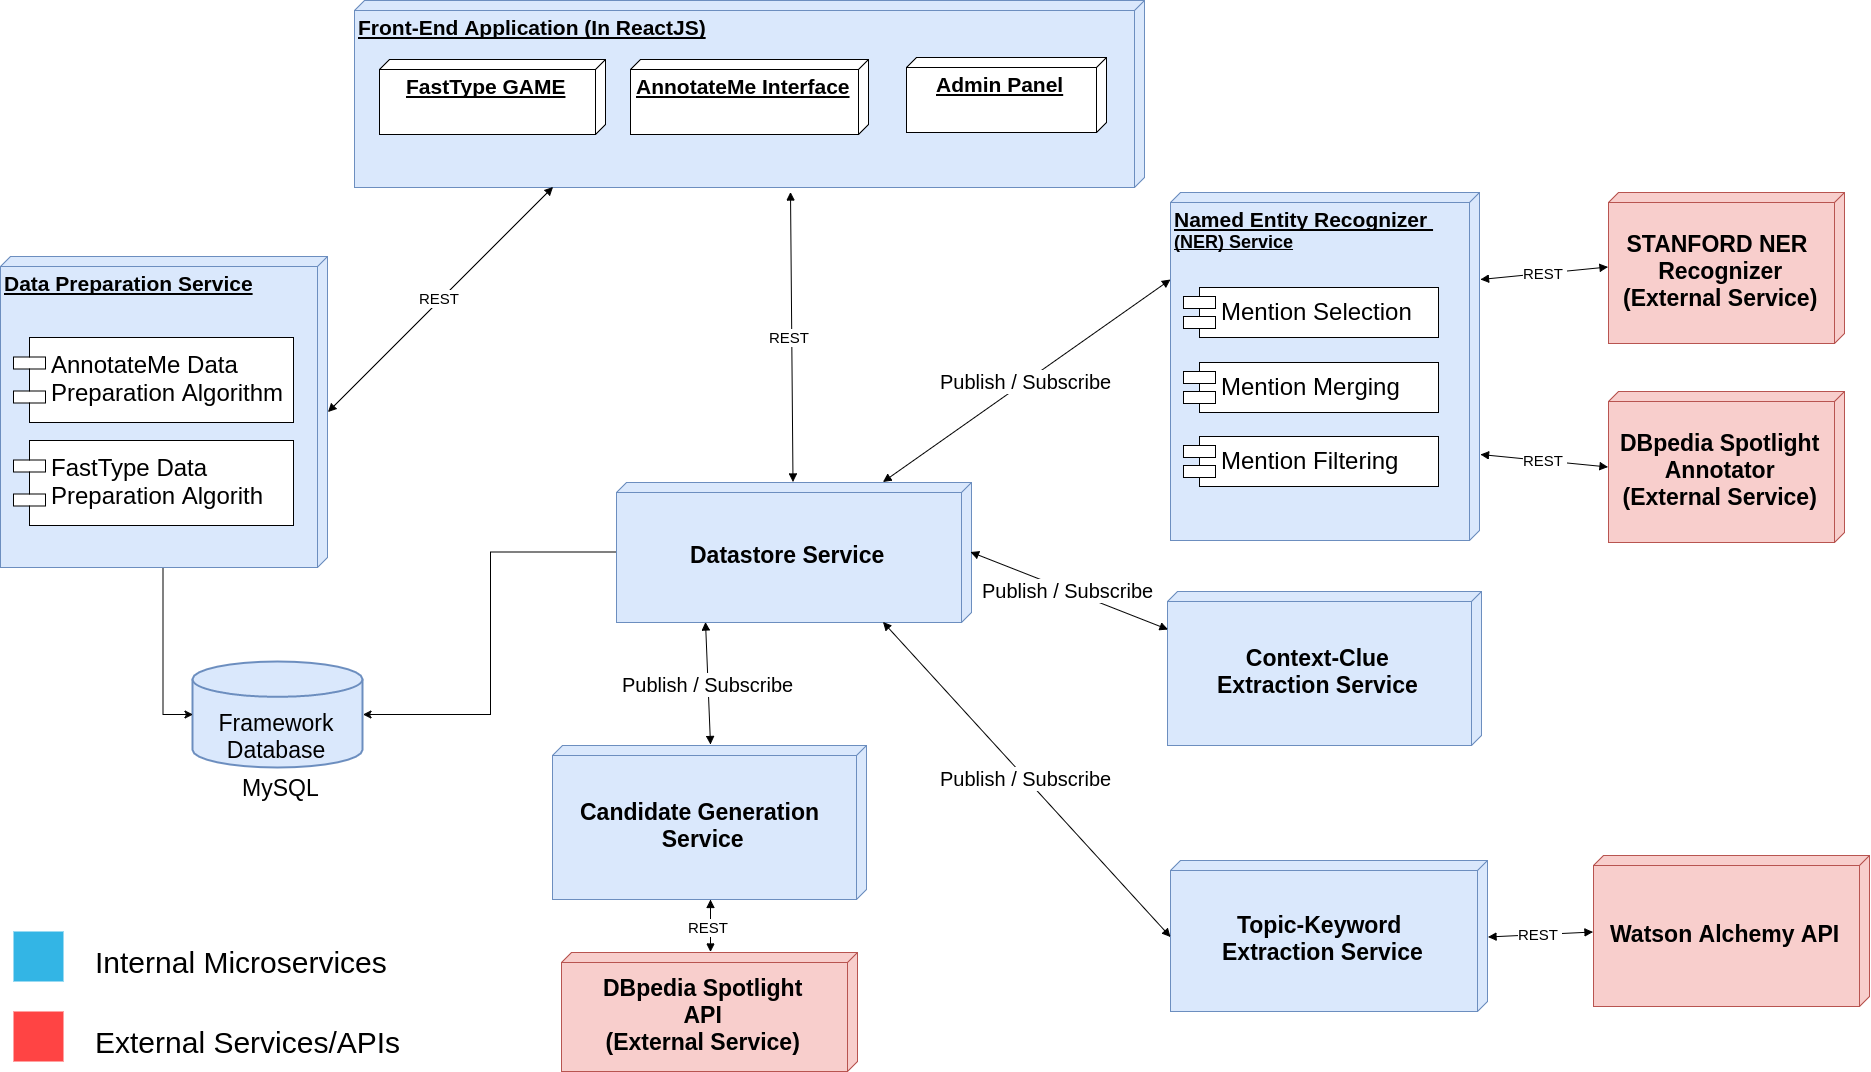
\includegraphics[width=\linewidth]{figures/microservice-architecture.png}
  \caption{Overview of the NED micro-service architecture}
  \label{fig:microservice_architecture}
\end{figure}

Observing the figure above, two different categories can be identified. The internal microservices (boxes highlighted with blue) are services that have been completely implemented from scratch. On the other hand, the external microservices (boxes highlighted in red) are external open source services that have been used by our framework to perform actions which were out of scope of this study. Among the external services, \textit{Stanford NER Recognizer} was the only external service that was not available as an online service offering API calls to perform the corresponding actions. A detailed explanation of the NER microservice is provided later in section \ref{framework:architecture_NER}.

%Communication Infrastructure
In a microservice architecture, a key factor that differs this architecture from other design patterns is the lightweight communication/messaging infrastructure. In our framework, we have utilized two different communication protocols, namely, Synchronous Messaging (\ac{rest}) and Asynchronous Messaging (\ac{amqp}). In cases where immediate response is required from a service to another, RESTful request/response API calls have been used to exchange information. We have tried to adhere to the fundamental rules of the RESTful messaging protocols where every functionality of the service is represented with a resource and operations carried out on top of these resources. As illustrated in Figure \ref{fig:microservice_architecture}, the front-end service which contains the admin panel, AnnotateMe Interface and Fastype Game communicate synchronously with the data preparation service and data store service. In addition to the front-end service, all external services are invoked using synchronous REST API calls since our internal microservices are not able to perform any internal actions unless the response from the external service is acquired. A complete documentation of the REST API calls implemented in the data store and data preparation services are available in Appendix \ref{appendix1:RESTDOCsec}.

Some of the services that compose the framework usually have a longer processing time compared to others because of the underlying complexity and the calculations that need to be performed. In these cases, it is more practical to use asynchronous messaging protocols without having to freeze the overall process as a consequence of one service which takes longer to complete. The publish and subscribe asynchronous message communication model was used for this purpose. More specifically, RabbitMQ \footnote{RabbitMQ Documentation Page \url{https://www.rabbitmq.com/documentation.html}} was used as the underlying lightweight message brooker based on \ac{amqp} (Advanced Message Queue Protocol). To see the different publishing and subscription routes that build the asynchronous communication infrastructure of the framework, see Appendix \ref{appendix1:AMQPDOCsec}.

%Conteinarization - Docker 
When designing a microservice architecture, among the many important design patterns that distinguish this architectural style from others is the deployment process. The deployment of microservices plays a critical role and when it comes to microservice architecture, the following key requirements have to be satisfied \cite{dzone}:
\begin{itemize}
    \item The ability to deploy/un-deploy independently each service
    \item It must be able to scale at each microservice level (as some services may experience more trafic than others)
    \item The ability to build and deploy microservices quickly
    \item In case one microservice fails to execute, other microservices should not be affected by this failure
\end{itemize}

To comply with the above mentioned requirements, Docker\footnote{Docker Documentation Page \url{https://docs.docker.com/}} was considered as the best microservice deployment solution. Docker is a containerization tool that lets developers and system administrators deploy self-sufficient application containers in Linux environments \cite{dzone}. Deploying a microservice into a docker container is as easy as writing a 5 line script. The steps involved to deploy an application into a docker container are as follows \cite{dzone}: 
\begin{itemize}
    \item Packaging the microservice as a Docker container image (usually by writing a script)
    \item Deploying each service instance as a container
    \item Linking containers with each other so that they are able to communicate (this is done automatically by Docker)
    \item Scaling is done by deploying many instances of the same container
    \item Building, deploying and starting a microservice is relatively fast as Docker uses containers instead of virtual machines (which is much slower compared to containers)
\end{itemize}

%Technology Stack - NodeJS, ReactJS, Mysql db
In terms of technology stack used to implement the microservice framework, the latest web technology tools have been utilized. In addition to the previously mentioned tools used for communication and deployment, the actual microservice applications framework has been implemented using NodeJS\footnote{NodeJS \url{https://nodejs.org/en/docs/}} as a back-end programming language, whereas for the front-end implementation we used ReactJS\footnote{ReactJS \url{https://facebook.github.io/react/}}. The combination of NodeJs and ReactJS has proven to be very efficient in terms of development speed, performance, agile development support and the incredible fast rendering capabilities which is very helpful during development and debugging of the application. As for the data storage, MySQL relational database has been used in our framework. 

Figure \ref{fig:workflow} illustrates the complete workflow of the framework. We use this illustration as a reference when describing the different services composing the framework in the following sections.


\begin{figure}[]
  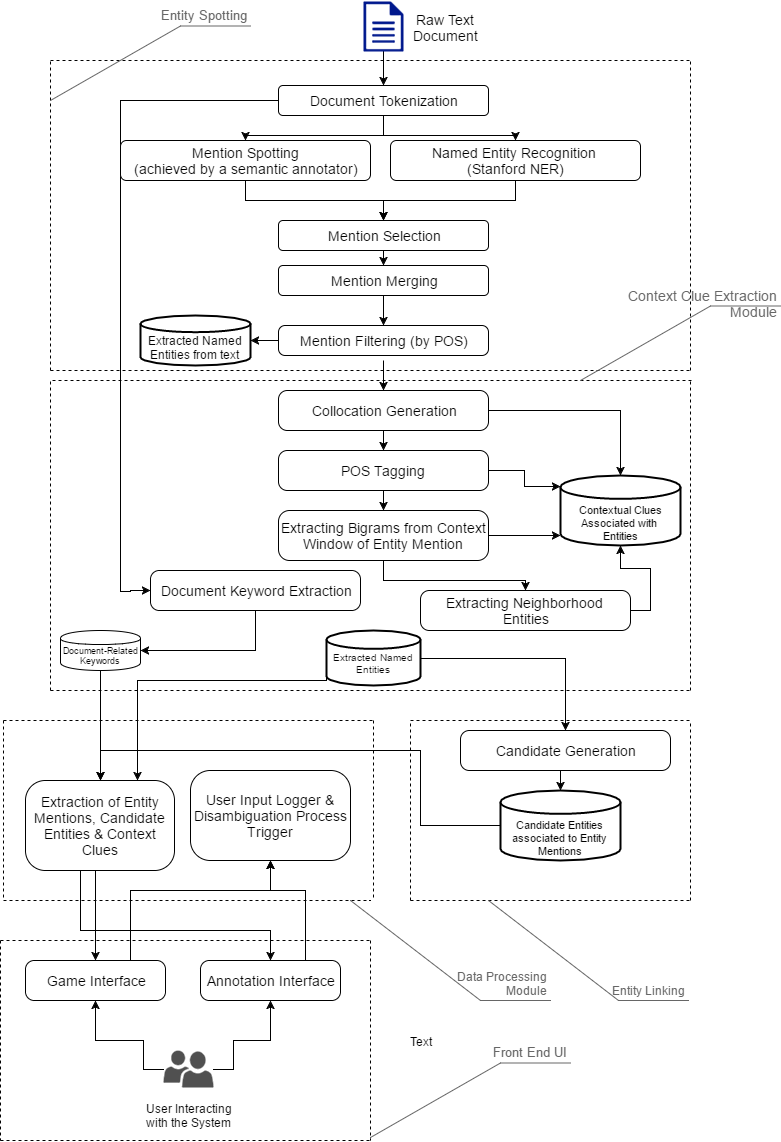
\includegraphics[width=\linewidth]{figures/workflow-diagram-v4.png}
  \caption{Overview of the complete workflow of the NED Framework}
  \label{fig:workflow}
\end{figure}


\newpage 
\subsection{Named Entity Recognition (\ac{ner}) Service}
\label{framework:architecture_NER}
The disambiguation process is initiated by uploading a raw text document through the admin panel which issues an API call to the data store service. The data store service persists the content of the document into the database and proceeds by publishing a \textit{named entity recognition} message which in turn is subscribed by the NER microservice. The published message contains all the textual content of the uploaded document. As can be seen in Figure \ref{fig:workflow}, the NER microservice starts by tokenizing the textual content of the document. A NodeJS implementation of a tokenizer has been used for this purpose \footnote{See Node Tokenizer \url{https://www.npmjs.com/package/tokenize-text}}. The tokenization process converts the text content into an array of words, sentences, characters or any other desired way. We use the tokenizer to split up sentences and individual words. 

The whole named entity recognition procedure has been inspired by \cite{39}, as they achieve very high levels of accuracy and significantly outperform state-of-the-art named entity recognizers. However, the implementation of the \ac{ner} service by Chabchoub et al. \cite{39} was carried out as part of the OKE Challenge 2016 and we were not able to find any open source code that could be integrated into our framework. Based on the information the authors provide in their publication, an attempted was made to reproduce the algorithms used in the recognition module in order to achieve similar performance levels as reported in their publication \cite{39}.

Stanford \ac{ner} \cite{standfordNER} has been used as a named entity recognizer in combination with Dbpedia Spotlight \cite{dbpedia} as a semantic annotator. Both (as external services) recognize the entities in the textual content and return a list of all the recognized entities. When comparing the results of each service, entity overlapping was observed. To be able to solve this, a selection algorithm is implemented in order to select the best entity out of both lists. The logic of the selection algorithm is keeping the longest mention and dismissing the short one. Lets take an illustrative example from the sentence below: 

\begin{quote}
\textit{"The State University of New York at Cortland celebrated its 149th anniversary this year."}
\end{quote}

In this example, Spotlight annotates \textit{State University} and \textit{New York}
 separately, whereas Stanford NER recognizes it as a single entity, namely, \textit{State University of New York}. The mention selection algorithm makes sure that the former is discarded and the later is kept. 
 
 However, even after the mention selection algorithm, it is not guaranteed that the correct entities have been identified. From the example sentence, in fact, the correct entity mention is \textit{State University of New York at Cortland}. In order to achieve this, the mention merging algorithm is performed. As explained by \cite{39}, given two named entities in close proximity, the algorithm will try to expand it to cover the next entity mention. The constraints checked by the algorithm to permit the expansion (avoiding pitfalls such as merging two legitimate different entities) have been described in detail by Chabchoub et al. \cite{39}. 
 
 The last step, before the entities are persisted into the database, consists of applying the mention filtering algorithm to the list of identified entities. The mention filtering algorithm uses a standard Part-of-Speech tagger for getting linguistic information for each entity. Accordingly, all entities that contain verbs are removed from the list, thus, filtering out incorrectly recognized entities \cite{39}. 
 
 The final result of the \ac{ner} micro-service contains a list of \textit{selected}, \textit{merged} and \textit{filtered} entities. The \ac{ner} service finalizes its process by publishing a \textit{named entity persist} message which is subscribed by the data store service that does the actual persisting of the entities into the MySQL database.

\subsection{Context Clue Extraction Services}
%Bigrams 
During the background chapter we emphasized the importance of context and how much it can affect the disambiguation accuracy for both, automatic and manual annotation systems. Referring back to the work-flow presented in the diagram in Figure \ref{fig:workflow}, contextual clues are extracted by following a three step process.

The process starts by removing all stop words in the sentences where the entity mentions are part of. After the stop words have been removed from the sentences, the \textit{collocation generation algorithm} is performed on those sentences. Collocations, according to Colson et al. \cite{52} represent the occurrence of two or more words within a short proximity between each other in text. They also argues that collocations are more likely to occur as fixed expressions such as compound nouns, proper nouns, idioms, noun-adjective combination, adjective-noun combination, verb-noun, well known song or film titles. The collocation generation algorithm follows these principles when deciding to keep a collocation from the sentence or not. Since we are dealing with analysis of grammatical structures in the sentence, part-of-speech tagging is a crucial step to be performed at this stage. 

After having extracted all potential collocations from the sentence provided as input data to the service, the next step is to associate these collocations as contextual clues to each and every entity. However, not every identified collocation within the sentence can be a useful context clue for the entity that is also part of that sentence. Previous studies have used a context window size of 4, which means that they take four preceding and four subsequent words from the sentence where the target entity occurs \cite{35}. The number 4 has been chosen because the accuracy of sense resolution does not improve when more than 4 words around the target word are considered. However, recent studies argue that the context windows size around the ambiguous target entity is dependent on the nature of the word itself \cite{35}. Our solution to this problem is increasing the context window size depending on how ambiguous the target word is. The ambiguity of a target entity is defined by the number of potential candidates extracted from the \ac{kb}. The more candidates are generated for the target entity, the higher the level of ambiguity. We believe that this represents an accurate metric on deciding the context size of the target entity. 

Since collocations can be a combination of more than two words, we have decided to keep only collocations that are composed of two words (i.e. bigrams). This decision is influenced on the findings acquired by Mihalcea and Rada \cite{36}. They observed that in terms of words in context, bigrams seem to be more effective than simple keywords and other combinations larger than two.In addition to the collocations which are considered as clues to help summarize the context in which the target word occurs, neighbour entities also also fall into this category. Since the algorithm has information on the exact position of each entity in the sentence (by maintaining a starting and ending index), we are able to decide which (other) entities are in close proximity to the target entity. Usually all identified entities that are part of the same sentence as the target entity are considered as neighbor entities. In some cases, when the sentence is short, the algorithm looks for neighbor entities in the preceding and subsequent sentences. The algorithm maintains a constraint on which it bases its logic whether to consider keeping or discarding a neighbor entity for the target entity. The constraint is basically a calculated word distance between the target entity and all other potential neighbor entities. 

After the local contextual clues have been extracted by our internal microservice, the last step is the extraction of document keywords. Document keywords are used to represent the theme or topic of the document, and might help in the disambiguation process in addition to local contextual clues. In this stage, Alchemy API is queried which extracts the most important keywords from a document. These keywords are associated as context clues to all identified entities in the same document whereas local context clues are distinct from one entity to another. Figure \ref{fig:context-clue} illustrates an example of a paragraph and the corresponding results after running the context clue extraction service. In this example, the target entity for which the context clues are to be associated is highlighted in red. The legend illustrated as a table in the example figure explains the meaning of the different colors. In cases where the words are underlined and highlighted with different colors, it means that the word combination has multiple purposes. For example "New York" from the illustrative paragraph in Figure \ref{fig:context-clue} is considered a neighbor entity to G1 (the target entity) in addition to being a keyword that contributes to understanding the meaning of the complete paragraph.


\begin{figure}[]
  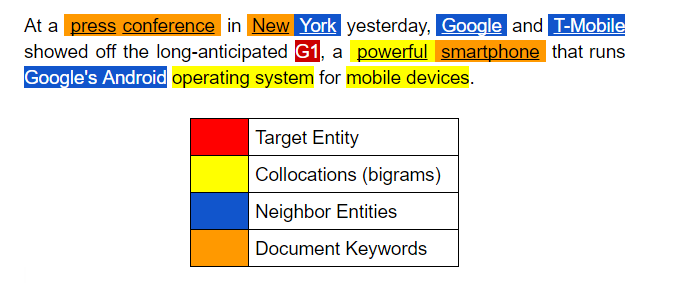
\includegraphics[width=\linewidth]{figures/context-clues.png}
  \caption{An example of a paragraph and the different contextual clues extracted from the service}
  \label{fig:context-clue}
\end{figure}

\subsection{Candidate Generation Service}
Dbpedia Spotlight is the semantic annotator which is queried by the \textit{Candidate Generation Service} to extract DBpedia candidates for a specific entity mention. No special logic has been applied in this service and therefore, the results retrieved after querying Dbpedia Spotlight are persisted into our system without additional modifications to the original data.

Dbpedia Spotlight \cite{dbpedia} performs the disambiguation process by pre-ranking entity candidates for each surface form spotted in the text. A combination of a prior score and a contextual score is calculated in order to determine which candidate entity is the most relevant. The prior score represents an estimation of how often the surface form is used as an anchor in a Wikipedia hyperlink that points to the entity page \cite{39}. Whereas the context score makes use of the context of the phrase (usually a window of words around the phrase) and the context of each candidate entity (calculated internally by Spotlight). When querying highly ambiguous entities such as "Paris" which can have over ten target candidates, only the best 8 are fetched to be evaluated. According to a user study conducted by Bontcheva et al. \cite{33}, participants gave feedback that having more than 8 options to choose from is associated with high cognitive load which results in immediately exhausting users. In addition to the maximum number of 8 candidate entities, we provide a last option called "none of them" in case the Spotlight was not able to fetch the correct candidate in the list.

During the experimental user study we observed that Spotlight was not able to provide the correct candidate entity for many entity mentions. Therefore we experimented with providing different context window sizes to the annotator to see if the performance changes. First we queried Spotlight by providing only the entity itself without any other contextual information. Second, the contextual clues extracted by our microservice were put in a sentence together with the target entity with clues located prior and after the target entity (based on where the clues were located on the original sentence). Finally, the original sentence where the target entity is part of, was used as context and sent as query parameter to Spotlight. We report in the results section of this chapter that the differences in performance between the three groups is relatively small and does not assure statistical significance.

\subsection{Data store \& data preparation service}
To assure the control and consistency of data being processed by the different microservices composing the framework, the \textit{Data-Store Service} was designed to be the only entry point to which the data could be manipulated. The service provides endpoints for accessing and manipulating the information residing on the database as a means of API calls and asynchronous message inquiries. It also serves as an information provider to the admin panel in the front-end application and also subscribes to different message routes such as: persisting named entities recognized from \ac{ner} microservice, persisting context clues and associating the generated candidate list to all registered entity mentions in the database. Besides subscribing to these message routes, the \textit{Data-Store Service} is the service endpoint that manages the complete asynchronous messaging infrastructure.

On the other hand, the \textit{Data-Preparation Service}, as the name implies, prepares the data for the AnnotateMe Interface as well as for the Fastype Game. Similar to the Data-Store Service, it has direct access to the database information with only one specific permission: reading (i.e. querying and retrieving information from the database). Therefore, for the sake of centralization and control of data, the Data-Preparation Service is considered as a read-only service with regards to the database access.

A unique feature implemented in the data preparation service is, as we like to call it, the \textit{disambiguation trigger}. This feature is responsible for resolving a specific entity mention (deciding which candidate represents the correct link for the target entity) when enough annotation data from the human annotators are accumulated. Since the most usual use-case scenario includes non-expert human annotators performing the validation process by either using the AnnotateMe Interface or the Fastype game, assuring quality of annotations is reached through redundancy. The level of redundancy maintained in the data preparation service is based on constraints proposed by Snow et al. \cite{32}. They conducted an experiment where they evaluated the quality of non-expert annotators in comparison with expert annotators. Their results indicate that on average it requires 4 independent non-expert annotations to achieve the equivalent ITA of a single expert annotator. Therefore, the disambiguation trigger is triggered when 4 independent annotations (having the same candidate as the selected option) have been accumulated for a specific entity mention. After an entity has been resolved, it will no longer show up on the interface for validation. The resolving step is done by the \textit{Data-Preparation Service} which initiates a REST API call to the \textit{Data-Store Service} in order to update the information on the databse.

%Order effects
A final element that is taken care by the \textit{Data-Preparation Service} is the ordering of candidates presented to human annotators. In a study conducted by Duarte et al. \cite{34}, they argue that in search engines, web users expect the best answer to be in the first or second position. This type of expectation represents potential bias on the results assessing the behaviour of annotators. After performing some user studies, they conclude that search result selection behaviour is influenced by ranking, with users showing tendency to select higher ranks without exploring other alternatives. To avoid having this situation in our experiment, we encourage users to explore all the candidates presented to them before making a decision. The encouragement is done by providing short descriptions for each candidate on the interface. Additionally, we avoid the chance of making users form assumptions about potential candidates being ranked higher in a list by completely randomizing the process of candidate positioning. Random positioning of alternatives instead of ranking has proven to be much more effective in encouraging users to explore all available alternatives instead of making blind decisions \cite{34}.


\newpage
\subsection{AnnotateMe Interface}

\begin{figure}[]
  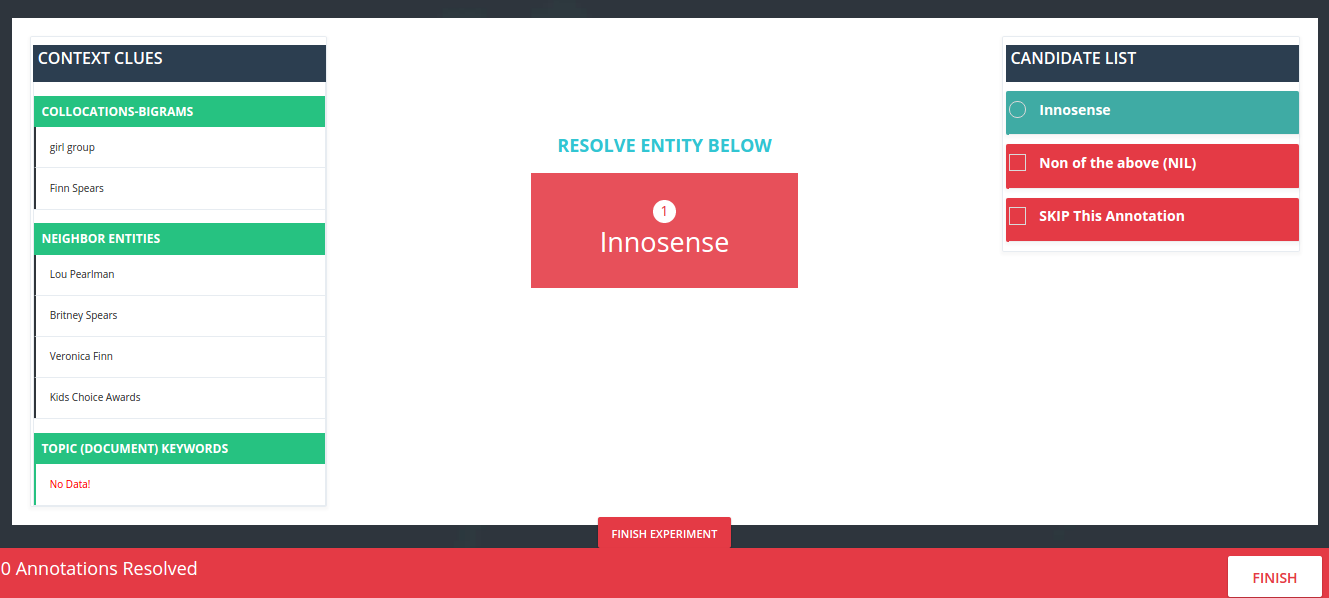
\includegraphics[width=\linewidth]{figures/annotateme-interface.png}
  \caption{The AnnotateMe Interface used to conduct the first experiment for validating the links generated by the NED Framework}
  \label{fig:annotateme-interface}
\end{figure}

During the implementation of the AnnotateMe Interface, we tried to come up with a simple UI and UX design of the interface in order to maintain low levels of complexity and avoiding confusion. Some of the design patterns identified by Hinze et al. \cite{15} necessary for non-expert users to annotate the presented content have been explored while implementing the annotation interface. These design patterns include:
\begin{itemize}
    \item Intuitive User Interface - an interface that is easy to grasp with actions that require minimal effort to discover and perform
    \item Simple Vocabularies - the current architecture of the framework provides annotations of entities within the categories of Organization, Location and People which are genuinely simple in nature.
    \item Focus on user task - The interface does not have any disruptive features or elements that would shift the focus of the annotator from its main task, that is, resolving the presented named entity.
\end{itemize}

% Quality check
According to Bontcheva et al. \cite{33} the single most influential part of any linguistic annotation exercise is the annotators ability to understand and conduct the annotation task. In order to achieve this, the guidelines and tools provided by the annotation interface play a major role in controlling such behavior. Presenting the user with simple, short guidelines that include examples and specific instructions on how to perform certain actions is very helpful. Additionally, having a clean interface is of utter most importance which contributes to an intuitive interaction during the annotation process. \cite{33} 

Figure \ref{fig:annotateme-interface} represents the design of the AnnotateMe Interface used for conducting annotations with non-expert users. The target entity mention to be resolved is presented in the middle of the page and attracts the users focus by reflecting its importance in the overall task. The contextual clues are presented to the right hand side of the interface and are grouped based on their origin of extraction. The right hand side of the interface is reserved for the candidate list. Each candidate can be expanded by clicking on its name. The expanded candidate provides the user with additional information that describes the meaning of the candidate (usually a short description). The two last options in the candidate section highlighted with red provide some degree of freedom to the user in case they are unfamiliar with the entity or when they think that the correct candidate is not provided in the list. These two options being discussed are: \textit{Non of the above(NIL)} and \textit{Skip this annotation}. The interface presented in Figure \ref{fig:annotateme-interface} has been used to conduct the first experiment which will be described in detail in the next upcoming section.
\newpage
\section{Methodology}
\label{framework:methodology}

The implementation of the Named Entity Disambiguation Framework with all its underlying microservices represent the tool which is used to study and answer the first two research questions. The majority of the implementation patterns and algorithms are based on theoretical background and reviewed literature on the respective field. In absence of open source code, the \ac service has been implemented as a reproduction of the work conducted by Chabchoub et al.~\cite{39}. However, without actual contribution of human annotators by participating in a user study, the answers to the research questions would not have been resolved. The first experimental user study has been conducted in order to get detailed insights on how well the information processed and presented to human annotators would contribute to generating annotation data. The reason that two user studies were conducted during this research work was to measure the engagement and playfulness of the game when compared to a standard, non-gamified interface for named entity disambiguation. Data from both experiments have been used to analyze and compare the different characteristics in order to draw on conclusions that we initially set to achieve. Regardless, this methodology section represents all the necessary information needed to successfully conduct the first experiment and describe the techniques and methodologies used to analyze the results.

%Datasets 
In order to conduct the annotation experiment by using the designed AnnotateMe Interface, an annotation data gathering process was conducted beforehand. In absence of linguistic and expert annotators to construct a gold standard which would have been used for assessing the quality of annotations, we decided to use already existing datasets, namely, Spotlight and KORE50 datasets \cite{datasets-ex1}. The first dataset contains documents from news articles whereas the second one contains short articles extracted from various domains. KORE50 is known by the NLP experts as a dataset characterized with a highly ambiguous nature. Table \ref{tab:experimentone_dataset} summarizes all the different entity types that are recognized in each dataset used in our evaluation experiment. As observed from the table, both datasets are composed mostly of entities in the three main categories: Organization, Location and People. The table was originally reported by Steinmetz et al. \cite{datasets-ex1}, and during the time of their writing, some of the entity mentions recognized in the dataset did not have a \ac{kb} representative. However, it has been mentioned that the information in \ac{lod} is continuously increased by researchers contributing with new datasets and extending existing ones, the ratio of mentions and entities from both datasets is likely to be more equalized now\footnote{The number of entity mentions recognized in the text having a corresponding \ac{kb} representative is increased.}. However, the analysis and results presented in the next section are up-to-date and take into consideration the latest versions of KROE50 and Spotlight datasets. 

\newpage
% Table generated by Excel2LaTeX from sheet 'Sheet1'
\begin{table}[htbp]
  \centering
  \caption{Distribution of entity types for Spotlight and KORE50 \cite{datasets-ex1}}
    \begin{tabular}{|l|rr|rr|}
    \toprule
    \multicolumn{1}{|c|}{\multirow{Class}} & \multicolumn{2}{c|}{Spotlight } & \multicolumn{2}{c|}{KORE50} \\
\cmidrule{2-5}          & \multicolumn{1}{l|}{Entities} & \multicolumn{1}{l|}{Mentions} & \multicolumn{1}{l|}{Entities } & \multicolumn{1}{l|}{Mentions} \\
    \midrule
    Total & 249   & 331   & 130   & 144 \\
    Agent & 1.40\% & 2.70\% & 66.90\% & 70.80\% \\
    -Organization & <1\%  & <1\%  & 19.40\% & 5.30\% \\
    --Company & <1\%  & <1\%  & 9.20\% & 9.70\% \\
    --Sports Team & -     & -     & 7.70\% & 6.90\% \\
    ---Socer Club & -     & -     & 7.70\% & 7.90\% \\
    -Person & 2.00\% & 2.40\% & 48.50\% & 51.40\% \\
    --Artist  & -     & -     & 17.70\% & 18.80\% \\
    ---MusicalArtist & -     & -     & 17.70\% & 18.80\% \\
    --Athlete & -     & -     & 6.90\% & 8.30\% \\
    ---SoccerPlayer & -     & -     & 5.40\% & 6.30\% \\
    --OfficeHolder & <1\%  & <1\%  & 4.60\% & 4.20\% \\
    Disease & 1.60\% & 1.20\% & -     & - \\
    EthnicGroup & 1.20\% & 1.80\% & -     & - \\
    Event & 1.20\% & <1\%  & -     & - \\
    Place & 10.40\% & 10\%  & 10.80\% & 10.40\% \\
    -Architectural Structure & 2.00\% & 1.50\% & 3.10\% & 2.80\% \\
    --Infrastructure & 1.60\% & 1.20\% & <1\%  & <1\% \\
    -PopulatedPlace & 7.20\% & 7.60\% & 5.40\% & 5.50\% \\
    --Country & 3.60\% & 3.30\% & -     & - \\
    --Region & <1\%  & <1\%  & -     & - \\
    --Settlement & 2.40\% & 3.30\% & 3.80\% & 3.50\% \\
    ---City & 1.60\% & 2.10\% & 2.30\% & 2.10\% \\
    Work  & <1\%  & <1\%  & 6.20\% & 6.30\% \\
    -MusicalWork & <1\%  & <1\%  & 3.10\% & 3.50\% \\
    --Album & <1\%  & <1\%  & 3.10\% & 3.50\% \\
    \bottomrule
    \end{tabular}%
  \label{tab:experimentone_dataset}%
\end{table}%

%recruiting participants
The participants who took part in the annotation experiment were invited through emails and social media. On the invitation message sent to all participants, a short and abstract description of the idea behind the experiment was provided. It is important to note that payment incentives and any other type of incentive which would degrade the voluntary participation of the user were avoided, thus assuring a complete voluntary participation without any beneficial intentions. As a result, 30 participants showed up and successfully completed the experiment.

The experiment was conducted in closed group rooms at the university campus in order to make sure that the participant was not being distracted while performing the experiment. Before starting to perform the actual annotations, the participants were presented with a consent form which explained the nature, purpose and intentions of the experiment. Participants were also fully aware that the participation was anonymous and voluntary and withdrawal from participation was possible at any time. The consent form for the first experiment is provided in Appendix \ref{appendix1:annotatme}.

On average, the duration of a single experiment session was about 25 minutes long. We also asked the participants to fill in a pre-questionnaire to gather demographic information about them as well as questions that assessed the level of expertise of each participant in the field of semantic web and natural language processing. In order to avoid potential biases on the results, we made sure that participants had moderate to native skills in English. We report on the demographic data of participants in the next section whereas the questions provided in the pre-questionnaire are presented in Appendix \ref{appendix1:annotatme}.

The non-expert nature of participants and the time constraints on the duration of an experiment session for each participant was the main reason for recording an instructional video to be presented to each participant before starting the actual annotation task. This video was essentially a replacement for an introductionary interface that is usually implemented for such experiments. During the 4 minute demonstrative video, we demonstrated to the participants how the interface is used and the purpose of each elements towards the general idea of annotating. After having read the consent form, filled in the pre-questionnaire and watched the demo video, the participants proceeded in doing the annotations for 15 minutes. However, the experimenter did not provide upfront information on how many annotations had to be performed. After the estimated 15 minutes elapsed, the participants were instructed to either finish the experiment or continue do more annotations This was a technique we used for measuring the level of enjoyment that participants had towards the interface. After the participant free-willingly\footnote{A free-will annotation is an annotation performed by a participant after being aware that the experiment was completed. This is a metric to measure the attractiveness of and engagement with the interface as perceived by the participant.} decided to finish the experiment, he or she was asked to fill in a post-questionnaire. The post-questionnaire contained questions with the purpose of assessing the quality, usability and engagement level of the interface. We report on the results of the post-questionnaire in the next section. The questions provided in the post-questionnaire can be found in Appendix \ref{appendix1:annotatme}.

% Assessment methodologies, f-measures, annova analysis, accuracy calcuations (for NER and Automatic annotator)
For assessing the performance of the framework in terms of entity recognition, user annotation quality and agreement level, we used metrics such as precision, recall, f-score and one way ANOVA analysis of variance. These assessment methodologies are commonly used in entity linking systems \cite{12}. Furthermore, to be able to assess the performance of our approach with state-of-the-art frameworks we have used a generic benchmark called GERBIL  originally developed by Usbeck et al. \cite{40}. GERBIL is a comparison tool for easily discovering the strengths and weaknesses of your implementation with respect to the state of the art in named entity disambiguation. The tool is open source and is an extensible framework that currently supports 9 different annotations on 11 different datastes within 6 different data types (recognition, disambiguation, linking etc). We report on the results of our framework with respect to the state-of-the-art annotators offered by GERBIL for Spotlight and KORE50 datasets. 

% Justify why we have used the following methodology. Why is it best fit for our study and answering our research questions

% Likely sources of BIAS
Concerning limitations and potential sources of bias, the methodology we used for our research study can be considered partially immune. For the sake of reproducability, we need to note that the participants who were invited through emails and social media were within the scope of the university campus. Consequently, one might argue that they might have been biased to participate in the experiment. Since this was seen as the only way of recruiting the participants in the pressure of time and space, we account this as a potential source of bias and address as a limitation of the recruitment methodology. However, we assure consistency with regard to participant recruitment since the same approach was used to recruit participants for the second experiment as well. Therefore, in case the results indicate increased engagement and motivation by using the game compared to the plain interface, we are able to claim that the improvements are acceptable since we remain consistent in the methodology. 

%Hypothesis 
\paragraph{Hypothesis}
The aim of the first experiment is to find out whether the implemented framework supports qualitative annotations by non-expert annotators. Therefore, we hypothesize that:

\begin{itemize}
    \item H1.1: By implementing the complete entity disambiguation pipeline as a framework, non-expert users will be able to perform annotations with a quality compared to expert annotators!
    \item H1.2: Short contextual clues are preferred towards complete sentences or paragraphs and as such provide sufficient information to make correct disambiguations! 
\end{itemize}



\newpage
\section{Results}
\label{framework:results}
The reason for performing the first experiment with the AnnotateMe Interface was to find out whether our approach of formulating and presenting the annotation data to a non-expert annotator for validation would result in creating high quality annotations. During this experiment we have also tested the performance of our NER service to see how well the recognition task is performed in addition to testing the performance of DBpedia Spotlight as the utilized automatic annotator. Below we report on the different aspects of the experiment.

\subsection{Participants}
The non-expert annotators who took part in the first experiment can be characterized as moderate users of text processing tools who have (on average) moderate experience with tagging of textual documents. Please note that tagging was explained to the users as the process of assigning a label or a textual description to a picture, video or categorizing a document. In some cases, the easiest way of explaining the tagging process to a participant was taking the concept of a \textit{hashtag} as an analogy to tagging. However, a \textit{hashtag} provides a higher degree of freedom since the tagging process is open while in our case the user is presented with options to choose from. Regardless, they both share the same conceptual idea. These questions were used to obtain a rough idea about the informal level of expertise of each participant in text processing respectively.

The average annotator was a 25 years old male student studying in the field of Computer Science with a good familiarity of text processing tools, moderate experience with tagging, acceptable level of familiarity with semantic web concepts who considered himself as above average when asked for his English language skills. Figure \ref{fig:ex1-preqestionnaire} presents the results of the questions asked to the participants during the pre-questionnaire. 

\begin{figure}[]
  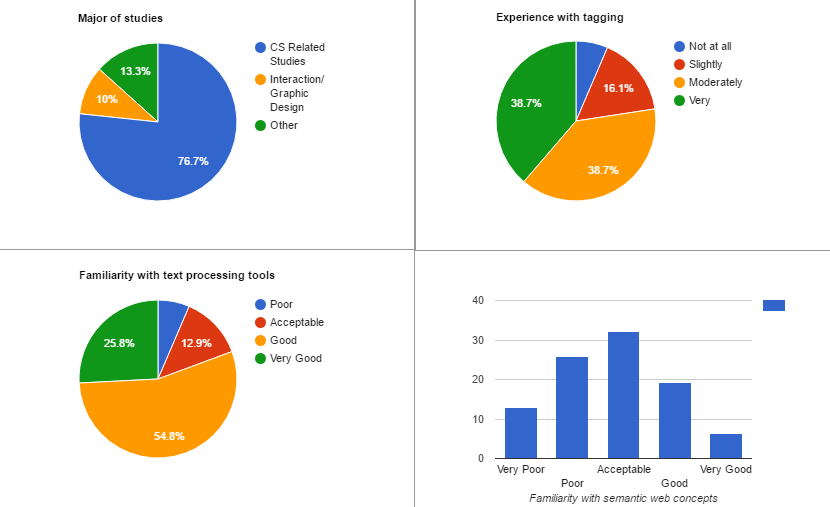
\includegraphics[width=\linewidth]{figures/experiment1/ex1-prequestionnairestats.PNG}
  \caption{Participant Statistics for Experiment 1}
  \label{fig:ex1-preqestionnaire}
\end{figure}

\subsection{NER Performance}
It has been mentioned earlier that the algorithms implemented in our \ac{ner} microservice are not novel solutions as opposed to the state-of-art. We attempted to reproduce the same algorithms used by \cite{39} since at the time of writing, their approach performed best compared to any other state-of-art \ac{ner} algorithms and tools. However, in absence of open source code, we tried to implement the service as similar as possible based on the information the authors provided in their white paper submitted at the OKE Challenge 2016 \cite{39}. As we can see from Table \ref{tab:ex1-nerperformance}, our framework performs significantly better than all the other automatic annotators for the KORE50 dataset, whereas for the spotlight we observe a slightly better improvement. Please note that we used GERBIL Benchmark \cite{40} to get the values for the other annotators whereas for our framework we calculated the same measures as explained by the benchmarking tool. 

% Table generated by Excel2LaTeX from sheet 'Sheet2'
\begin{table}[htbp]
  \centering
  \caption{NER Performance of automatic annotators in two datasets compared to our framework}
    \begin{tabular}{|l|ccc|ccc|}
    \toprule
    \textbf{-/Dataset} & \multicolumn{3}{c|}{\textbf{Spotlight Dataset}} & \multicolumn{3}{c|}{\textbf{KORE50 Dataset}} \\
    \midrule
          & \multicolumn{1}{l|}{\textbf{Precision}} & \multicolumn{1}{l|}{\textbf{Recall}} & \multicolumn{1}{l|}{\textbf{F-Score}} & \multicolumn{1}{l|}{\textbf{Precision}} & \multicolumn{1}{l|}{\textbf{Recall}} & \multicolumn{1}{l|}{\textbf{F-Score}} \\
    \midrule
    \textbf{Babelfy} & 0.22  & 0.18  & 0.19  & 0.55  & 0.55  & 0.53 \\
    \textbf{Dbpedia} & 0.61  & 0.34  & 0.43  & 0.73  & 0.23  & 0.27 \\
    \textbf{AIDA} & /     & /     & /     & 0.64  & 0.53  & 0.57 \\
    \textbf{Dexter} & 0.71  & 0.27  & 0.38  & 0.27  & 0.15  & 0.18 \\
    \textbf{AnnotateMe } & \textcolor[rgb]{ 1,  0,  0}{\textbf{0.69}} & \textcolor[rgb]{ 1,  0,  0}{\textbf{0.42}} & \textcolor[rgb]{ 1,  0,  0}{\textbf{0.49}} & \textcolor[rgb]{ 1,  0,  0}{\textbf{0.87}} & \textcolor[rgb]{ 1,  0,  0}{\textbf{0.8}} & \textcolor[rgb]{ 1,  0,  0}{\textbf{0.82}} \\
    \bottomrule
    \end{tabular}%
  \label{tab:ex1-nerperformance}%
\end{table}%

Our intentions were to see how good our framework performs when dealing with entities that have a very high ambiguous nature (KORE50 Dataset) but also with entities that have moderate levels of ambiguity (Spotlight Dataset). However, the number of entities present in each dataset was relatively big and resolving all of those entities using the framework would require running the experiment for longer periods. Therefore we used only a subset of documents from the Spotlight Dataset wheres for the KORE50 dataset we used all the available documents. For reproducability reasons, the following documents from the Spotlight dataset were considered: Arts1, Business1, Fashion1, Medicine1, Music1, Privacy1, Science1, Sports1, Travel1 and Travel2. The complete dataste is available online at the GERBIL website \footnote{\url{http://aksw.org/Projects/GERBIL.html}}. The total number of recognized entities by our NER microservice was 208 with 77 being entities recognized from the Spotlight dataset and 131 entities recognized from the KORE50 dataset.


\subsection{Annotation Quality and Performance}
Among the 208 total recognized entities by our \ac{ner} microservice, only 82 of them were resolved during the first experiment. It should be emphasized again that for one entity to be resolved we required 4 unique judgements from different participants to agree on one specific candidate for it to be resolved. We measured the performance of the human annotators, DBpedia Spotlight and other automatic annotators on those 82 resolved entities and evaluated whether the candidate associated with the entity was the correct one based on the gold standard. Additionally, since we wanted to see how DBpedia Spotlight (as our utilized automatic annotator) disambiguates entities based on the amount of contextual information surrounding the target entity, we report on three cases, namely: providing only the entity itself without any context information, providing the complete sentence and providing the contextual clues extracted from our framework. 
% Table generated by Excel2LaTeX from sheet 'Sheet3'
\begin{table}[htbp]
  \centering
  \caption{Annotation Results of AnnotateMe Interface and Dbpedia Spotlight Anntator}
    \begin{tabular}{|cc|cc|}
    \toprule
    \multicolumn{4}{|c|}{\textbf{Experiment 1 (Entity Name Only)}} \\
    \midrule
    \multicolumn{1}{|r|}{} & \multicolumn{1}{l|}{\textbf{All Datasets}} & \multicolumn{1}{l|}{\textbf{Spotlight Only}} & \multicolumn{1}{l|}{\textbf{KORE50 Only}} \\
    \midrule
    \multicolumn{1}{|c|}{\textbf{Correct (\%)}} & \multicolumn{1}{r|}{44.57} & \multicolumn{1}{r|}{72.22} & \multicolumn{1}{r|}{32.23} \\
    \multicolumn{1}{|c|}{\textbf{Incorrect (\%)}} & \multicolumn{1}{r|}{55.43} & \multicolumn{1}{r|}{27.78} & \multicolumn{1}{r|}{67.77} \\
    \midrule
    \multicolumn{4}{|c|}{} \\
    \midrule
    \multicolumn{4}{|c|}{\textbf{Experiment 1 (With Sentances)}} \\
    \midrule
    \multicolumn{1}{|r|}{} & \multicolumn{1}{l|}{\textbf{All Datasets}} & \multicolumn{1}{l|}{\textbf{Spotlight Only}} & \multicolumn{1}{l|}{\textbf{KORE50 Only}} \\
    \midrule
    \multicolumn{1}{|c|}{\textbf{Correct (\%)}} & \multicolumn{1}{r|}{51.38} & \multicolumn{1}{r|}{70.37} & \multicolumn{1}{r|}{43.31} \\
    \multicolumn{1}{|c|}{\textbf{Incorrect (\%)}} & \multicolumn{1}{r|}{48.62} & \multicolumn{1}{r|}{29.63} & \multicolumn{1}{r|}{56.69} \\
    \midrule
    \multicolumn{4}{c}{} \\
    \midrule
    \multicolumn{4}{|c|}{\textbf{Experiment 1 (With Context Clues \& Neighbor Entities)}} \\
    \midrule
    \multicolumn{1}{|r|}{} & \multicolumn{1}{l|}{\textbf{All Datasets}} & \multicolumn{1}{l|}{\textbf{Spotlight Only}} & \multicolumn{1}{l|}{\textbf{KORE50 Only}} \\
    \midrule
    \multicolumn{1}{|c|}{\textbf{Correct (\%)}} & \multicolumn{1}{r|}{54.24} & \multicolumn{1}{r|}{66.67} & \multicolumn{1}{r|}{48.78} \\
    \multicolumn{1}{|c|}{\textbf{Incorrect (\%)}} & \multicolumn{1}{r|}{45.76} & \multicolumn{1}{r|}{33.33} & \multicolumn{1}{r|}{51.22} \\
    \midrule
    \multicolumn{4}{|c|}{} \\
    \midrule
    \multicolumn{4}{|c|}{\textcolor[rgb]{ 1,  0,  0}{\textbf{AnnotateMe}}} \\
    \midrule
    \multicolumn{2}{|c|}{\textcolor[rgb]{ 1,  0,  0}{\textbf{Correct (\%)}}} & \multicolumn{2}{c|}{\textcolor[rgb]{ 1,  0,  0}{\textbf{Incorrect (\%)}}} \\
    \midrule
    \multicolumn{2}{|c|}{\textcolor[rgb]{ 1,  0,  0}{\textbf{88.46}}} & \multicolumn{2}{c|}{\textcolor[rgb]{ 1,  0,  0}{\textbf{11.53}}} \\
    \bottomrule
    \end{tabular}%
  \label{tab:exp1-annotatorRes}%
\end{table}%


Table \ref{tab:exp1-annotatorRes} presents the ratio of correctly and incorrectly linked entities by Dbpedia Spotlight. In general, the performance increased after providing more contextual information to the automatic annotator, which is an expected outcome. However, against our expectations, in the case of Spotlight Dataset, the ratio of correctly linked entities decreased after providing additional context information to the annotator. Despite the fact that the difference between the groups is not statistically significant for p < 0.5, it leads us to the assumption that Dbpedia Spotlight requires more content than just short contextual clues in order to make use of their internal techniques for disambiguation such as link probability, commonness, semantic similarity and other vector features relevant to context. Finally, we compare our performance results with other automatic annotators aside from Spotlight and we observe a significant improvement on both datasets. Table \ref{tab:exp1-annotatos-comparison} reports on the F-score of each annotator compared to our framework. 

Additionally, we run one-way Anova analysis of variance between two groups, namely, annotation results performed by non-expert users using the AnnotateMe Interface and results obtained by Dbpeida Spotlight automatic annotator. Statistically significant differences for p = 0.05 are obtained. As a result we claim that the non-expert annotators performed significantly better compared to other semantic annotators with an observed accuracy of 0.92 for the f-measure. Based on these results, the first hypothsis (H1.1) is strongly supported.

% Table generated by Excel2LaTeX from sheet 'Sheet4'
\begin{table}[htbp]
  \centering
  \caption{Comparison of AnnotateMe with other state-of-art semantic annotators}
    \begin{tabular}{|l|r|r|r|}
    \toprule
    \multicolumn{4}{|c|}{\textbf{Precision, Recall, F-Scores (Spotlight \& KORE50 Dataset)}} \\
    \midrule
    \textbf{Annotator} & \multicolumn{1}{l|}{\textbf{Precision}} & \multicolumn{1}{l|}{\textbf{Recall}} & \multicolumn{1}{l|}{\textbf{F-Score}} \\
    \midrule
    \textcolor[rgb]{ .8,  0,  0}{\textbf{AnnotatMe}} & \textcolor[rgb]{ .8,  0,  0}{\textbf{0.95}} & \textcolor[rgb]{ .8,  0,  0}{\textbf{0.88}} & \textcolor[rgb]{ .8,  0,  0}{\textbf{0.92}} \\
    \midrule
    Babelfy & 0.56  & 0.46  & 0.51 \\
    \midrule
    Dbpedia Spotlight & 0.53  & 0.39  & 0.44 \\
    \midrule
    Dexter & 0.27  & 0.17  & 0.2 \\
    \midrule
    WAT   & 0.55  & 0.41  & 0.46 \\
    \bottomrule
    \end{tabular}%
  \label{tab:exp1-annotatos-comparison}%
\end{table}%

In order to answer our second research question regarding context and deciding whether to accept or reject our second hypothesis (H1.2), we asked participants in the post questionnaire whether the contextual clues were helpful during the annotation process. They were also asked whether they would prefer to have the complete sentence as a representative of the surrounding context of the entity or whether they would prefer the short context clues already provided in the annotation interface. The results from the post questionnaire analysis show that 66.67\% of the participants preferred the short context clues as opposed to the 31.25\% of the other group who said that they would prefer sentences instead. To see whether contextual clues really helped on the disambiguation process for those participants who approved them as helpful clues, we calculated the level of agreement of each participant. The level of agreement is a simple calculation that takes the number of correct entities resolved and divides it by the total number of annotations performed. Results show that from the group who agreed having short contextual clues rather than sentences, on average they agreed with other annotators 54.47\% of the time, while those who preferred sentences agreed on average 48.44\% of the time. We observe a slight improvement on the agreement level in this case. Figure \ref{fig:ex1-agreementlevel} presents the overall agreement levels of all participants who took part in the first experiment. The average agreement level for all participants is 51\%. Please note that this does not represent a 50-50 chances of agreeing with another participant. In most cases, when resolving an entity, each participant was presented with 8 options in addition to the 9th option being "none of the above". Therefore, a 51\% reported agreement level can be considered a good performance. However, the difference between the agreement level reported for the group who preferred context clues compared to those who preferred sentences is not statistically significant for p = 0.05 and as a result our second hypothesis is rejected. 

%agreement level
\begin{figure}[]
  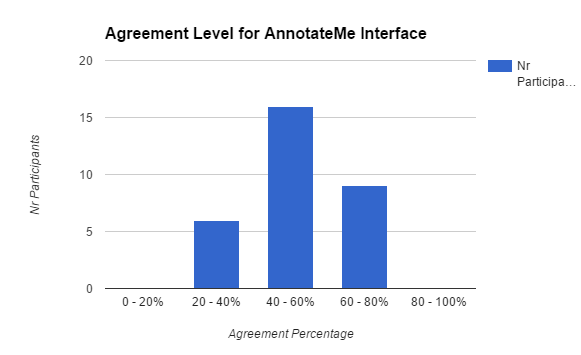
\includegraphics[width=\linewidth]{figures/experiment1/exp1-agreementlevel.PNG}
  \caption{Participants' Agreement level for the first experiment}
  \label{fig:ex1-agreementlevel}
\end{figure}
 

%freewill annotations
The setup of the first experiment was designed in a way that each individual participant performed annotations for 15 minuets constantly. They were not told upfront that they will be performing such tasks for 15 minutes, but were instructed to do the task until the experimenter told them to stop. After the estimated time elapsed they were asked whether they would like to continue do more annotations or stop and conclude the experiment. Participants were not encouraged to do any annotations after the 15 minute time trial had passed, thus the rest of annotations performed were completely voluntary and considered as free-will annotations. On average, each participant performed 22 annotation rounds during those 15 minutes. In terms of free-will annotations, one participant performed 17 annotation rounds on average. These results are used later to compare with the gamified system in order to assess the perceived engagement as a measure of time spent performing \textit{free-will annotating}. 

On the post questionnaire we asked participants to evaluate their experience with the task, the usability of the interface and perceived engagement. Figure \ref{fig:ex1-postresults} reports the results on the different questions asked on the post questionnaire. It can be concluded that the participants perceived the task to be interesting and somewhat engaging with a possibility that the participants would continue perform such task in the future. Regarding the usefulness of contextual clues, the graph indicates that users perceived the clues on average as useful when disambiguating a named entity. In addition to that, we report also on the perceived frustration while performing the task. Figure \ref{fig:ex1-frustration} indicates that the participants were seldom frustrated during the annotation process with some of the participants reporting to having been frustrated about half of the time. This can be an outcome of the participants being not familiar with the entities since they did not have the freedom of choosing a specific category or genre during the first experiment. 

%post questionnaire results 
\begin{figure}[]
  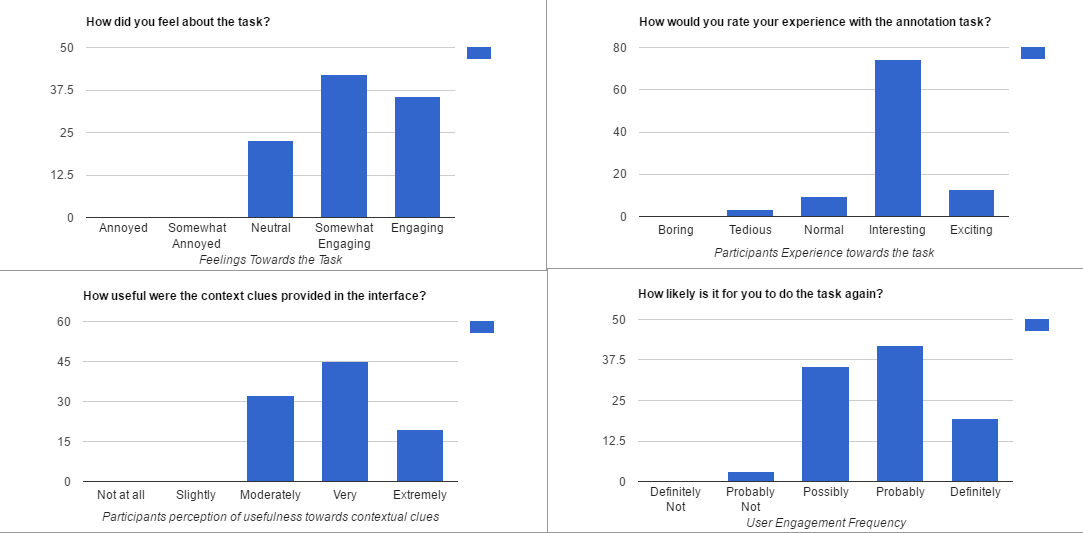
\includegraphics[width=\linewidth]{figures/experiment1/ex1-postquestionnaire.PNG}
  \caption{Experiment 1 Post Questionnaire Results}
  \label{fig:ex1-postresults}
\end{figure}

\begin{figure}[]
  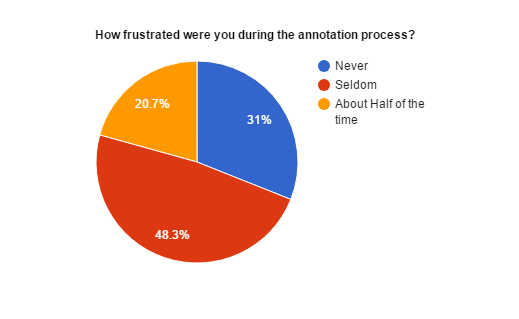
\includegraphics[width=\linewidth]{figures/experiment1/ex1-frustration.PNG}
  \caption{Reported level of frustration experienced during the annotation process}
  \label{fig:ex1-frustration}
\end{figure}

%Short contextual clues are preferred towards complete sentences or paragraphs and they provide sufficient information to make correct annotation decisions!

%What the chapter said - conclude the chapter